\section{ExtRA Framework}
\label{sec:method}

\begin{figure*}[th]
	\centering
	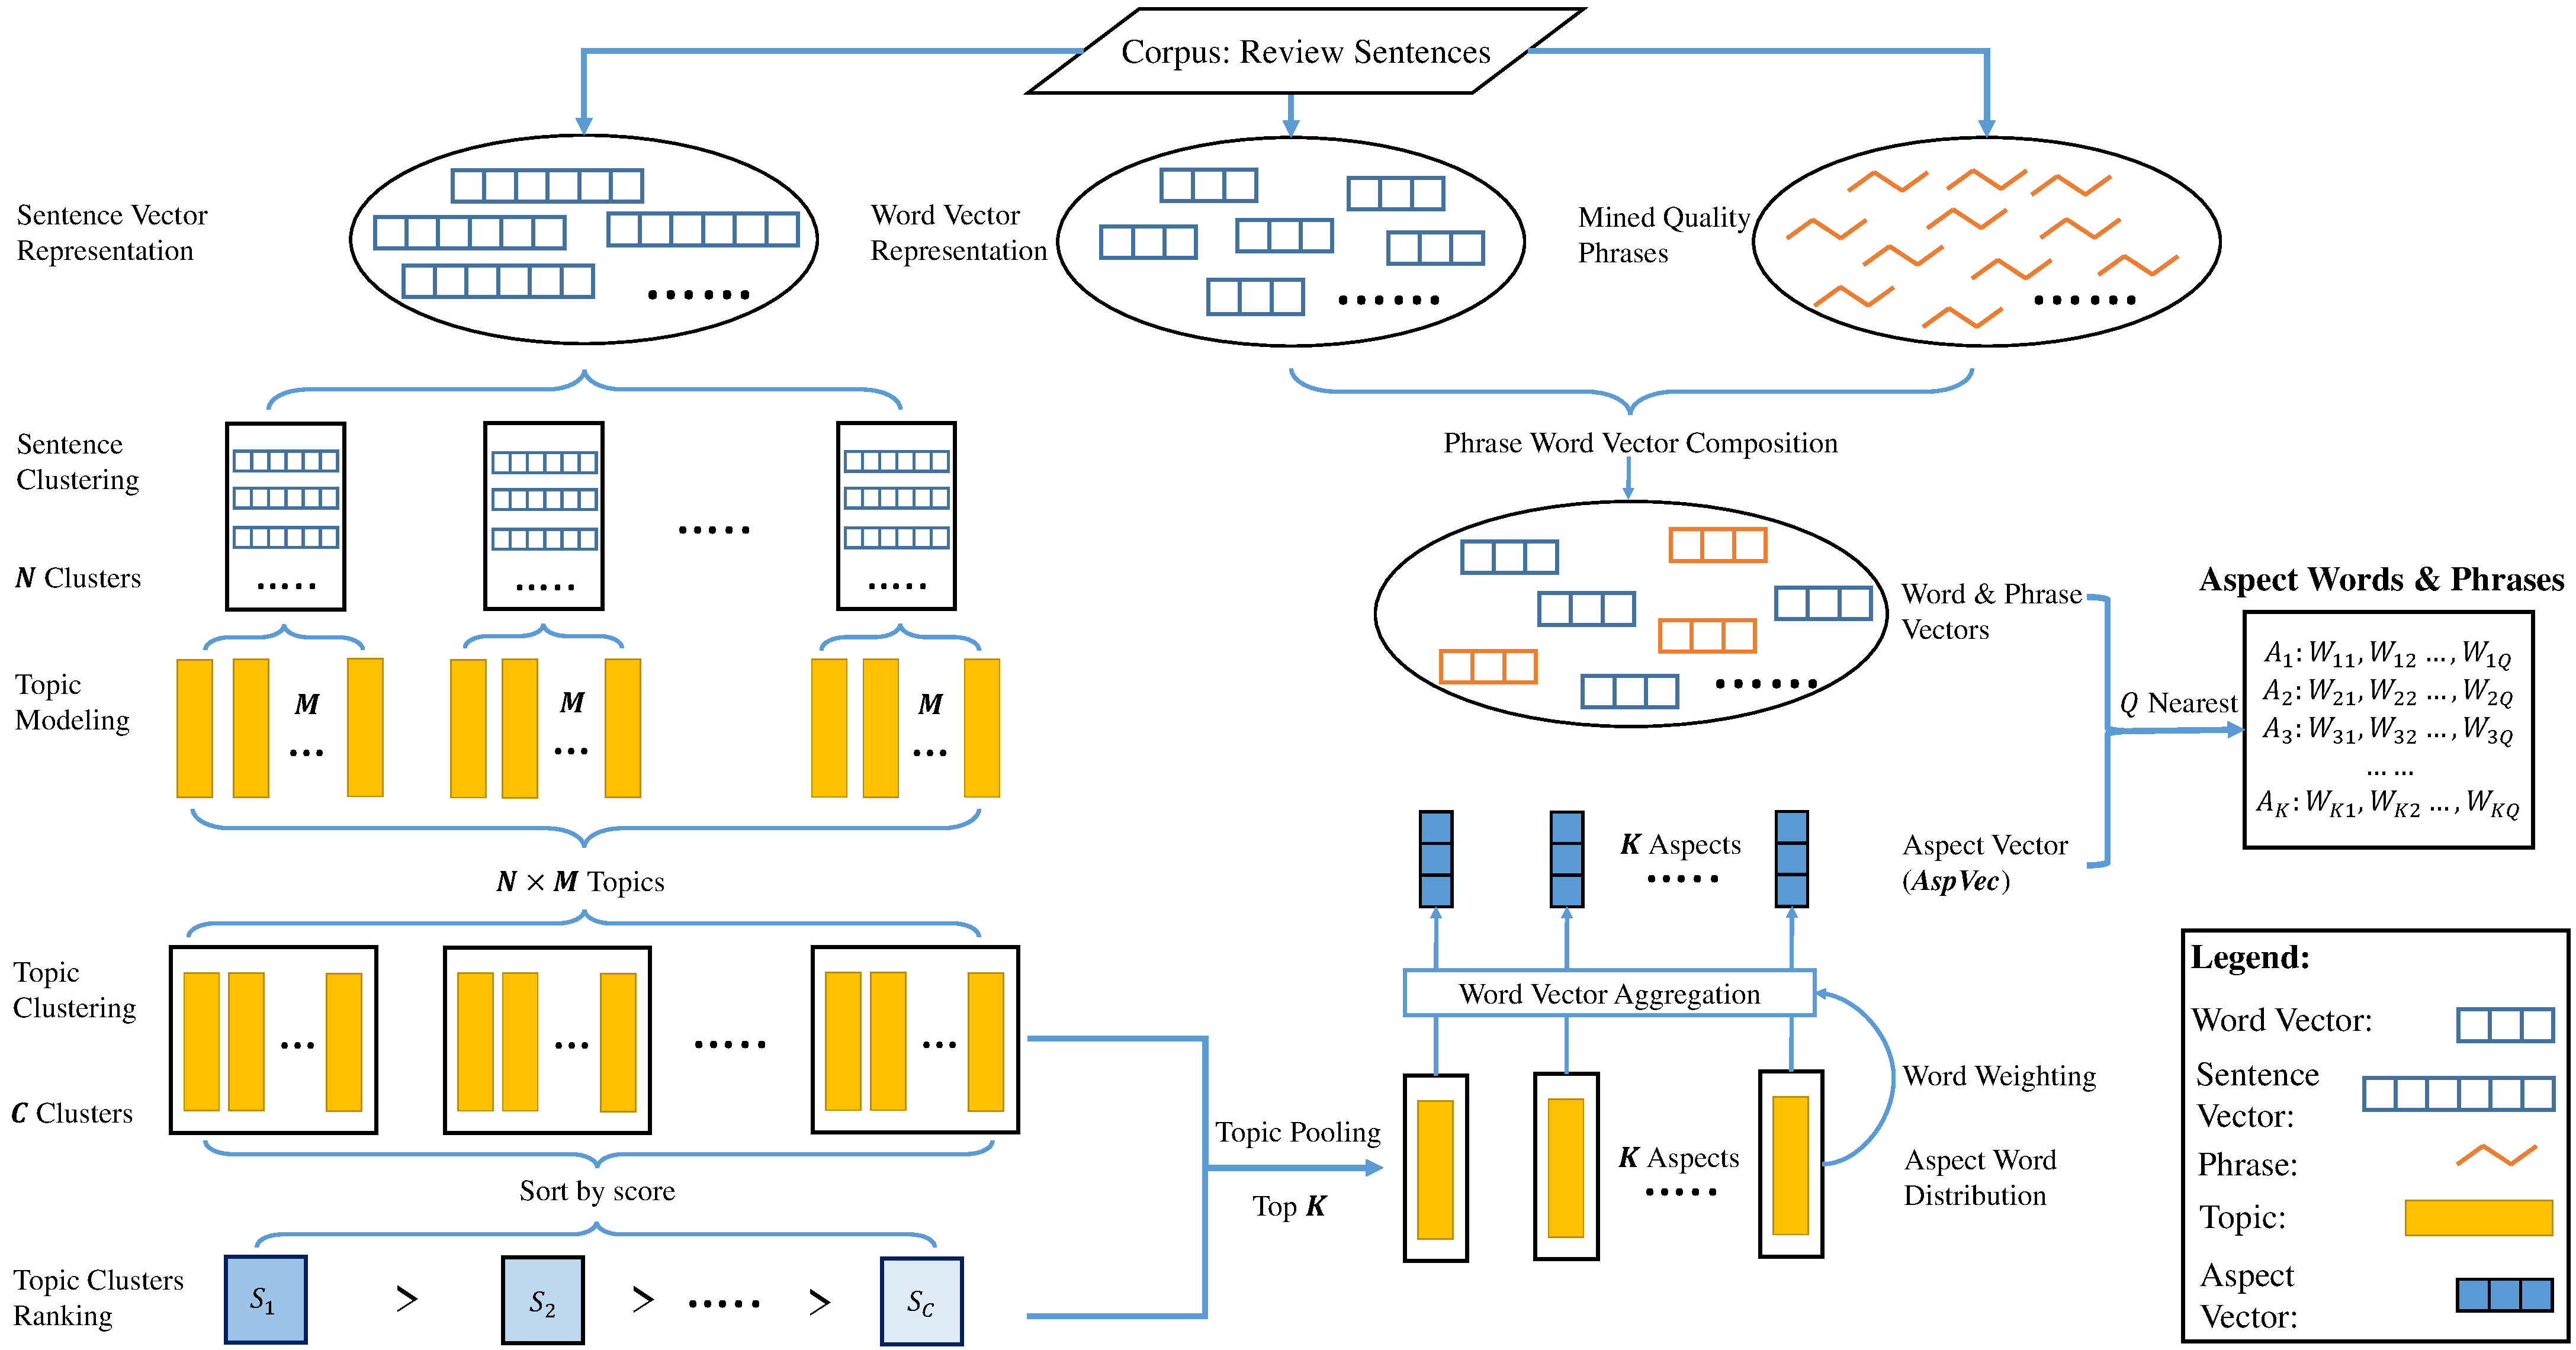
\includegraphics[width=\textwidth]{figures/overview}
	\caption{Our overall framework.}
	\label{fig:framework}
\end{figure*}

The review aspect extraction problem aims to extract $K$ noun words or phrases 
from user reviews about a given type of product,
each of which should represent a distinct aspect or feature of particular product or service type. 
Here $K$ is an constant parameter for the problem. 
The set of reviews and the number of aspects are inputs.
%Note that in this definition we don't use cross-domain information, 
%that is, for one product type we only use the reviews of that domain.
%Thus, our model can extract aspects across domains with ease.
%This allows us to apply the model to any domain with ease.
The overall workflow of ExtRA framework is shown in \figref{fig:framework} which consists of 5 stages. 
We will discuss the motivation and details of each stage in following subsections.
%\BL{we can briefly introduce the 5 stages here in the preamble}

\subsection{Stage 1: Sentence Representations and Clustering}

%For user reviews, many topics can be compressed into a short paragraph and
%each topic corresponds to a potential aspect of the product.
A typical hotel review extracted from \figref{fig:tripadvisor} 
is shown below. We can see that topics (underlined) in this review 
can shift very quickly, and
the adjacent sentences may refer to 
completely different aspects about a product. 
Plus, sentences about the same review aspect may not 
appear consecutively in a review. 

\begin{quote}
\textit{\underline{Pool} is small and only 4 ft but refreshing. \underline{Hot tub} also there. \underline{Staff} were super friendly each day. \underline{Room} was nothing special but clean and comfy. Lots of \underline{restaurants and bars} nearby. \underline{Breakfast} was great and despite being a busy weekend there was always a big selection available.''}
\end{quote}
%we convert each sentence in the reviews into a vector representation 
%and cluster them in to $N$ clusters of semantically similar sentences.


Such fine-grained semantic shifts in user reviews 
make it difficult to simply apply the bag-of-word  
and normal topic modeling on reviews.
Therefore we propose to work on sentence level instead 
of document level, and it would be helpful if we can divide long
reviews with multiple aspects into several centered topic-oriented review segments.

Motivated by this observation, the first stage of our framework is to perform
sentence clustering.  
Instead of using simplistic methods like bag-of-word representation, 
we leverage distributed representation which encodes words and sentences as low-dimensional real-valued vectors.
Existing  sentence representation methods include averaging word vector in a sentence, ParagraphVector (PV)\cite{le2014distributed}, LSTM-based RNN\cite{hochreiter1997long} trained for language modeling etc.

After obtaining sentence representations,
we cluster them into $N$ clusters by k-means algorithm\cite{kmeans}.
%We then collect the similar sentences from a review and
%each review document is divided into several shorter documents, each belonging
%to one of the $N$ clusters. 
As a result, we obtain $N$ clusters of sentences sharing similar semantics.

\subsection{Stage 2: Topic Modeling}

%To isolate the noises that exist in the sentence cluster,
%for each sentence cluster we further generate $M$ 
%topics, resulting in $N\times M$ different word distributions in total.
%Sentence clustering step clustered semantical similar sentences together. 
%However, each cluster may still mix up with multiple aspects. 
Although we performed sentence clustering based on semantic sentence representations, there exit some sentences in the obtained cluster that may still mix up with some noise and overlapping aspects.
For example, the following two sentences are taken from two TripAdvisor reviews. 
Sentence A) mentions multiple aspects such as {\em room}, {\em staff} and {\em price}. 
Sentence B) is only about the {\em location} aspect however lexically it seems to be talking about food.
Thus, it is also difficult for sentence representations like PV to correctly determine the aspects in these sentences. 
As a result, each cluster contains multiple aspects and there are also overlapping across clusters. 

\begin{quote}
A) \textit{``The room was clean, the staff were friendly, and I would say the price is very reasonable given the proximity to business and leisure destinations around downtown.''}
\end{quote}

\begin{quote}
B) \textit{``There is a restaurant just 5 min walk away with nice Italian food, pizza was great.''}
\end{quote}

%Fengshi: The result is overlaps between clusters about 
%different aspects and noises within each cluster.

To isolate the aspects and resolve such overlaps between short review pieces, we propose to perform traditional topic modeling in each cluster of sentences.
We apply the state-of-the-art Biterm Topic Model (BTM) \cite{cheng2014btm} topic modeling within each sentence cluster and generating $M$ smaller topics for each cluster. 
This will give us in total $N\times M$ topics (word distributions). 
BTM is a word co-occurrence based topic model that learns topics by modeling word-word co-occurrences patterns (i.e., biterms). In contrast, LDA and PLSA are word-document co-occurrence topic models, since they model word-document co-occurrences.
A biterm consists of two words co-occurring in the same context, for example, in the same short text window. Unlike LDA models the word occurrences, BTM models the biterm occurrences in a corpus. In generation procedure, a biterm is generated by drawn two words independently from a same topic. In other words, the distribution of a biterm $b=(w_i,w_j)$ is defined as:
\begin{equation}
	P(b) = \sum_k{P(w_i|z)*P(w_j|z)*P(z)}.
\end{equation}
With Gibbs sampling algorithm, we can learn topics by estimate $P(w|k)$ and $P(z)$.

\tabref{table:overlap} shows an example of topics inferred from $N=3$
sentence clusters with $M=5$ from hotel reviews and illustrates the overlap problem.
In this example, five topics (t1-t5) were extracted from each sentence cluster, 
and each row is one topic. 
It can be seen that the aspects for those 
three clusters should be {\em room}, {\em location} and {\em price} 
respectively.
However, topics shown in boldface font obviously belong to 
other clusters.  Especially, the last topic of the third cluster 
appears to be an overlap of more than two clusters.
This topic modeling extracts multiple topics from each cluster, and each topic indicates the potential expected aspect.

\begin{table}[th]
	\centering
	\caption{Topics extracted from three sentence clusters of hotel review.}
	\label{table:overlap}
	\begin{tabular}{|c|l|}
		\hline
		& t1: room bed bedroom size floor \\
		Sentence
		&t2:  bedroom room wall size decor \\
		cluster 1
		&t3:  room bathroom shower water towel \\
		&t4:  room suite size view floor \\
		&t5:  room shower area kitchen bed \\\hline
		
		&t1:  station minute tube location bus \\
		Sentence
		&t2:  location price night place rate\\
		cluster 2
		&t3:  location square station street subway\\
		&t4:  distance bus subway downtown shopping\\
		&t5:  \textbf{restaurant} \textbf{city} \textbf{food} \textbf{buffet} \textbf{place} \\\hline
		
		&t1:  price rate service money star\\
		Sentence
		&t2:  \textbf{location} \textbf{city} \textbf{star} \textbf{time} \textbf{rate} \\
		cluster 3
		&t3:  price service night money city\\
		&t4:  price location place night city\\
		&t5:  \textbf{location} \textbf{service} \textbf{food} \textbf{price} \textbf{restaurant} \\\hline
	\end{tabular}
\end{table}


\subsection{Stage 3: Topic Clustering}
\label{sec:topic_clustering}

To address the above problems, we propose to take a step forward and cluster the topics across the sentence clusters, which means we are supposed to cluster the previous $N*M$ clusters into $C$ topic clusters.
Here $C$ is purposely set to be larger than $K$ for that we would like to pruning them into $K$ aspects later.
%We treat each topic as a vector, where an entry is the frequency of a word. 
%These vectors have dimensionality equal the size of the vocabulary, which is too large for clustering, 
%so we perform dimensionality reduction these vectors.
%Specifically, we use PCA to reduce the topics vectors to 100-dimensional. 
%By doing this, we select the 100 most important components that best distinguish different topics.
We represent each topic as a topic vector which is actually the weighted sum of word vectors using $p(w|t)$ as weights, 
among top $k$ dominant words with highest $p(w|t)$ probabilities.
Such topic vectors represents the topic centers by integrating the topic word semantics. 
%Then we perform k-means algorithm on the $N\times M$ topic vectors to 
%generate $C$ topic clusters.
%We need to set $C$ slightly larger than 
%the desired number of product aspects $K$, due to the overlapped topics as shown 
%in \tabref{table:overlap}.
Thus, the noisy topics can be clustered together and later discarded. 
We evaluate the quality influence of these redundant clusters on 
final aspects in our experiments.

\begin{table}[th]
\caption{Aspect clusters extracted from hotel reviews.
Each row shows the candidate words of an aspect, sorted by the weight of each word.}
\label{table:step3}
\centering
\begin{tabular}{|l|} \hline
breakfast, meal, food, tasty, dinner, morning, coffee, tea \\\hline
room, night, time, bed, day, bathroom, staff, area, place \\\hline
staff, desk, service, friendly, reception, concierge, helpful \\\hline
close, city, location, place, central, station, bus, street\\\hline
bed, shower, spacious, room, size, bathroom, bedroom, floor \\\hline
price, room, check, night, money, city, location, star, service \\\hline
location, price, room, night, place, rate, money, time, city  \\\hline
\end{tabular}
\end{table}

Finally, for each cluster we take the mean of the $(N\times M)/C$ topics and normalize it
for the word distribution of that cluster.
We call them {\em aspect clusters}.
Some example aspect clusters extracted from hotel reviews are 
shown in \tabref{table:step3}.

\subsection{Stage 4: Aspect Cluster Ranking}
In previous steps, we formed $C$ aspect clusters including some noisy clusters supposed to be removed.  
We propose a {\em distinctiveness score} to measure the cluster quality which captures 
the intuition that the more the cluster overlaps with others the lower distinctiveness score associates to it, which indicates a lower quality of the cluster. 
Thus, we discard $C-K$ noisiest clusters. 
For the $i$th cluster $C_i$ ($i\in [1, C]$), 
the distinctiveness score $S(i)$ is defined as following:
\begin{align}
S(i) &= \sum_{w\in C_i} S_i(w) \nonumber\\ 
     &= \sum_{w\in C_i} \log\left(\frac{f_i(w)}{\sum_{j\neq i} f_j(w)}\right)\nonumber, \\
\end{align}
where $f_i(w)$ represents the significance score of word $w$ in cluster $C_i$ which is the sum of the weights of $w$ from topic $t$ (e.g. $v_t(w)$) in $C_i$, computed as following: 
\begin{equation}
    f_i(w) = \sum_{t\in C_i} v_t(w)
\end{equation}
Subsequently, the clusters are ranked in the descending order of 
this score and the last $C-K$ clusters are discarded.
The result is shown in \tabref{table:clustersranked}, 
the discarded cluster are grayed-out.

\begin{table}[th]
\caption{Aspect clusters ranked by distinctiveness score.
Potential aspect words are boldfaced.}
\label{table:clustersranked}
\centering
\begin{tabular}{|l|} \hline
\textbf{staff}, desk, \textbf{service}, friendly, reception, concierge, helpful \\\hline
breakfast, meal, \textbf{food}, tasty, dinner, morning, coffee, tea \\\hline
\textbf{price}, room, check, night, money, city, location, star, service \\\hline
bed, shower, spacious, \textbf{room}, size, bathroom, bedroom, floor \\\hline
close, city, \textbf{location}, place, central, station, bus, street \\\hline
\textcolor{mygray}{room, night, time, bed, day, bathroom, staff, area, place} \\\hline
\textcolor{mygray}{location, price, room, night, place, rate, money, time, city} \\\hline
\end{tabular}
\end{table}

\subsection{Stage 5: Aspect Generation}
\label{sec:word_ranking}
After previous cluster ranking stage, we obtain $K$ aspect 
clusters, each of which represents a potential aspect. 
We aims to extract top aspect candidates from those clusters.
We have two methods toward this goal. One is a word ranking algorithm
which only produces a list of aspect words, the other is an embedding
based aspect term encoder-decoder algorithm that uses a
vector representation known as AspVec and produces both words
and phrases. 

\subsubsection{Word Ranking}
%We propose a word ranking approach for each aspect cluster, and extract the top word as the aspect from each aspect cluster.
%After previous cluster ranking stage, we obtain $K$ expected aspect clusters, each of which associates with a quality score.
In this subsection, we propose a word ranking approach to indicate the most prominent words in each aspect cluster. After such ranking, we can simply select the top-ranked word 
as aspect words. We refer this method as {\em ExtRA-Words}.

In \tabref{table:clustersranked},
we manually boldfaced the most representative words for each cluster.  
Each of them is the expected aspect word which can be treated as 
a summary of other words in the same cluster.
However, it can be seen that not all of them have the highest frequency 
in their clusters.  
In order to automatically select the best aspect words,
we propose a word ranking step to adjust the order of word in aspect cluster by considering both the weights and semantics of words.
%Since each aspect cluster contains a bunch of topics generated after topic modeling stage, the weights of words can be calculated in each cluster.
%We keep only nouns from this step since the appropriate aspects 
%should be nouns. 
We design our ranking metric to capture prominence of words in aspect cluster.
Intuitively, the most prominent and representative word in each cluster
is assumed to be the closest to centroid of the aspect cluster.
Therefore, we calculate the semantic similarity of each word with all other 
words in the cluster and use that to measure how central that word is.
To calculate the semantic similarity between two words, 
we use the cosine similarity of word embeddings. 
Word2Vec is a very popular 
word embedding model and has been shown to perform well on 
the semantic similarity tasks \cite{levy2015improving}.

%In this word ranking step, we not only rank the words in each cluster so that
%the top word is the most prominent to that cluster, 
%we also want to make sure that such top-ranking words do not appear in
%multiple clusters, as it would be inappropriate to have duplicate aspects. 
In order to prevent generating duplicate aspects from different aspect cluster,
we process the clusters in a sequential order, based on the ranking given by the previous step of aspect cluster ranking. 
When we calculate the score for word $x$ the $i$th cluster $C_i$,
we also consider the scores of word $x$ in cluster 1 to $i-1$, 
where the scores have already been calculated. 
We prevent the duplicate aspect words by subtracting the scores 
of other clusters from the score of cluster $i$.
The score of word $x$ in the $i$th cluster $C_i$ is thus defined by:
\begin{equation}
s_i(x) = u_i(x) \sum_{y\in C_i}\hat{x}\cdot \hat{y} - \sum_{j=1}^{i-1}s_j(x),
\label{eq:wordscore}
\end{equation}
where $\hat{x}$ is the vector representation of x; $u_i(x)$ is the weight of $x$ in cluster $C_i$.
The words in each cluster is ranked by this score following the order given by cluster ranking.
This gives us the final aspect clusters. 
The effect of duplicate prevention is evaluated in the next section.

\subsubsection{Aspect Term Encoder-Decoder} % Aspect Vector generation
In order to consider multi-word aspects, we extend our vocabulary with high quailty phrases extracted by AutoPhrase\cite{liu2017phrase}. 
We propose a method to encode words, phrases and aspect clusters into the same vector space.
Therefore, we can compute the similarity between them with ease.

After word ranking step, each word associates a representative score in each aspect cluster. 
We encode  aspect clusters as vectors named {\em AspVec}, by taking top T ($T=50$) most representative words in each aspect cluster and summing up their embeddings weighted by corresponding normalized word ranking score $w_c(x)$. 
{\em AspVec} integrates the prominent word semantics together, representing the semantic of aspect cluster as following:
\begin{equation}
w_c(x) = \frac{s_c(x)}{\sum_{y\in V_T}s_c(y)}
\end{equation}
\begin{equation}
AspVec(c) = \sum_{t=1}^T{w_c(x)E(x)},
\end{equation}
where $c$ is the aspect cluster, $V_T$ is the vocabulary of top T words, $x,y$ are words in $V_T$, and $E(x)$ is the embedding of $x$.

We also encode the phrase ($p$) vector representation ($E(p)$) in the same vector space, averaging the embedding of words in the phrase. 
\begin{equation}
E(p) = \sum_{x\in p}{E(x)}
\end{equation}
In such way, we encode the aspect cluster centers and surface terms including words and phrases into the same vector space. It is natural to select terms nearest to cluster center as the aspects. 
Nor aspect candidates include both words and phrases. 
We find the semantically nearest words or phrases for the aspect cluster in order to decode $AspVec$ into representative surface terms.
Therefore, we search Q-Nearest neighborhoods for particular aspect cluster, i.e. $AspVec$, harvesting a ranking list.
We pick the top-ranked candidate as the final extracted aspect.

%\subsubsection{Aspect Term Decoder}
%In this section, 
%Futhermore, we propose a method to calculate the vector representation for each aspect cluster and introduce phrases candidates using AutoPhrase. 








